\documentclass[../main.tex]{subfiles}


\usepackage{nopageno} %Seitenzahlen auf richtiger Seite 

\usepackage[left=2cm, right=2cm, top=2cm, includehead, includefoot, headheight=17pt]{geometry}

\usepackage[utf8x]{inputenc}
\usepackage[english]{babel}
\usepackage{amsmath,amssymb,amsthm}
\usepackage{framed}
\usepackage{wasysym}
\usepackage[T1]{fontenc} %Silbentrennung 
\usepackage{color} %Farbe
\usepackage{graphicx}
\usepackage{float}%Grafik am gleichen Ort plazieren
%pdf. png. einfach eingliedern
\usepackage{subfigure} %Grafiken nebeneinander
\usepackage{pdfpages}
\usepackage{ulem} 	%\uuline{urgent}    % doppelt unterstreichen
%\uwave{boat}      % unterschlängeln
%\sout{wrong}       % durchstreichen
%\xout{removed}     % ausstreichen mit //////.

\usepackage{tikz}
\usetikzlibrary{trees}
\usetikzlibrary{plotmarks}
\usetikzlibrary{angles,quotes,babel}
\usetikzlibrary{shadings}
\usetikzlibrary{patterns}
\usetikzlibrary{matrix}
\usetikzlibrary{arrows}
\usetikzlibrary{calc}

\usepackage{pgfplots}
\usepackage{pgf-pie}
\pgfplotsset{compat=1.10}
\usepgfplotslibrary{statistics}
\usepgfplotslibrary{fillbetween}

\usepackage{tkz-euclide}
\usepackage{enumerate}
\usepackage{stmaryrd}
\usepackage{tabularx}
\usepackage{wrapfig}
\usepackage{epsdice}
\usepackage{multirow}
\usepackage{rotating}
\usepackage{pdflscape}
\usepackage{fancyhdr}

\pagestyle{fancy} %eigener Seitenstil
\fancyhf{} %alle Kopf- und Fußzeilenfelder bereinigen
\fancyhead[L]{} %Kopfzeile links
\fancyhead[C]{} %zentrierte Kopfzeile
\fancyhead[R]{} %Kopfzeile rechts
\renewcommand{\headrulewidth}{0.4pt} %obere Trennlinie
\fancyfoot[C]{\thepage} %Seitennummer
\renewcommand{\footrulewidth}{0.4pt} %untere Trennlinie

% Number spaces 
\newcommand{\CC}{\ensuremath{\mathbb{C}}}
\newcommand{\RR}{\ensuremath{\mathbb{R}}}
\newcommand{\QQ}{\ensuremath{\mathbb{Q}}}
\newcommand{\ZZ}{\ensuremath{\mathbb{Z}}}
\newcommand{\NN}{\ensuremath{\mathbb{N}}}
\newcommand{\LL}{\ensuremath{\mathbb{L}}}
\newcommand{\DD}{\ensuremath{\mathbb{D}}}
\newcommand{\WW}{\ensuremath{\mathbb{W}}}

%draw chemestry molecules 
\usepackage{chemfig} % https://mirror.ox.ac.uk/sites/ctan.org/macros/generic/chemfig/

\newcommand\vv[1]{%
	\begin{tikzpicture}[baseline=(arg.base)]
		\node[inner xsep=0pt] (arg) {$#1$};
		\draw[line cap=round,line width=0.45,->,shorten >= 0.2pt, shorten <= 0.7pt] (arg.north west) -- (arg.north east);
	\end{tikzpicture}%
} %command will render \vv{x} with an arrow aboth 

\renewcommand{\labelenumi}{\roman{enumi})}

\DeclareMathOperator{\ggT}{ggT}
\DeclareMathOperator{\sign}{sign}

%sections
\theoremstyle{plain}
\newtheorem{Thm}{Theorem}[section]
\newtheorem{Def}[Thm]{Definition}
\newtheorem{Prop}[Thm]{Proposition}

\theoremstyle{definition}
\newtheorem{lemma}[Thm]{Lemma}
\newtheorem{corollary}[Thm]{Corollary}
\newtheorem{claim}[Thm]{Claim}
\newtheorem{Proof}[Thm]{Proof}
\newtheorem{Ex}[Thm]{Example}

\newtheorem{Exercise}{ex}[section] %follow proper enum
\newtheorem{ex}[Exercise]{Exercise}
\newtheorem{Solution}{sol}[section]
\newtheorem{sol}[Solution]{Solution}

\theoremstyle{remark}
\newtheorem{remark}[Thm]{Remark} % follows thm enum

\newtheorem{comment}{Comment}[section] %follow comment enum
\newtheorem{notation}[comment]{Notation}
\newtheorem{reasoning}[comment]{Reasoning}
\newtheorem{Intpr}[comment]{Interpretation}

%some premmade with title (uterwise use \textbf{Title} ...)
\newenvironment{ThmWithTitle}[1]{%
	\begin{Thm}[\textbf{#1}]}{\end{Thm}}
\newenvironment{PropWithTitle}[1]{%
	\begin{Prop}[\textbf{#1}]}{\end{Prop}}
\newenvironment{ExWithTitle}[1]{%
	\begin{Ex}[\textbf{#1}]}{\end{Ex}}
\newenvironment{DefWithTitle}[1]{%
	\begin{Def}[\textbf{#1}]}{\end{Def}}
\newenvironment{RemarkWithTitel}[1]{%
	\begin{remark}[\textbf{#1}]}{\end{remark}}

%format of paragraph 
\renewcommand\paragraph{\@startsection{paragraph}{4}{\z@}%
	{-2.5ex\@plus -1ex \@minus -.25ex}%
	{1.25ex \@plus .25ex}%
	{\normalfont\normalsize\bfseries}}
\makeatother
\setcounter{secnumdepth}{4} % how many sectioning levels to assign numbers to
\setcounter{tocdepth}{4}    % how many sectioning levels to show in ToC

\newcounter{row} 
\renewcommand\therow{\alph{row}} %hier a,b,c etc. def und mit therow abrufbar

\newenvironment{aufz}
{\setcounter{row}{0}%
	\par\noindent\tabularx{\linewidth}[t]
	{\cdot{20}{>{\stepcounter{row}\makebox[1.5em][l]{\therow)\hfill}}X}} %bis max 20 Elemente nebeinander
}
{\endtabularx}


%biblio
\usepackage[]{biblatex}
\addbibresource{referenzenma.bib} 

%glossary
\usepackage{glossaries}
\usepackage{import}


\usepackage{rotating} % Include this package in the preamble

\newglossaryentry{exocytosis}{
	name=exocytosis,
	description={A cellular process in which substances contained in vesicles are released from the cell to the extracellular environment by fusion of the vesicle with the plasma membrane}
}

\newglossaryentry{endocytosis}{
	name=endocytosis,
	description={A cellular process in which the cell membrane folds inward to form a vesicle that encloses extracellular material for internalization into the cell. Or it can also describe the pathway by which material is transported inwards from the plamsa membrane}
}

\newglossaryentry{AP2}{
	name=AP2,
	description={An adaptor protein complex involved in clathrin-mediated endocytosis. AP2 binds to specific phosphorylated phosphoinositides in the plasma membrane}
}

\newglossaryentry{BARdomain}{
	name=BAR domain,
	description={A structural domain found in proteins that bind to and stabilize curved membranes. BAR domains can sense or induce membrane curvature and are involved in various trafficking pathways, including clathrin-mediated endocytosis}
}

\newglossaryentry{dynamin}{
	name=Dynamin,
	description={A large GTPase involved in clathrin-mediated endocytosis. Dynamin assembles around the neck of budding vesicles and, through GTP hydrolysis, facilitates membrane scission to release the vesicle into the cytosol}
}

\newglossaryentry{Rab}{
	name=Rab protein,
	description={A family of small GTPases that regulate vesicle transport by ensuring specificity in vesicle targeting. Rab proteins recruit effector molecules that help guide vesicles to the correct membrane compartment}
}

\newglossaryentry{SNARE}{
	name=SNARE protein,
	description={A group of membrane-associated proteins that mediate the fusion of vesicle and target membranes. SNAREs on the vesicle (v-SNAREs) and on the target membrane (t-SNAREs) form complexes that bring membranes close enough to fuse}
}

\newglossaryentry{NSF}{
	name=NSF,
	description={N-ethylmaleimide-sensitive factor; an ATPase that disassembles SNARE complexes after membrane fusion. NSF uses energy from ATP hydrolysis to recycle SNARE proteins for further rounds of vesicle fusion}
}

\newglossaryentry{homotypicfusion}{
	name=Homotypic membrane fusion,
	description={A type of membrane fusion in which two membranes of the same type or origin (e.g., two endosomes) fuse together. This process is important for organelle maturation and requires matching sets of SNARE proteins on both membranes}
}

\newglossaryentry{VTC}{
	name=Vesicular tubular clusters,
	description={Homotypic membrane fusio of ER-derived vesicles. They function as intermediate sorting stations that mediate cargo transport from the endoplasmic reticulum to the Golgi apparatus}
}

\newglossaryentry{KDEL}{
	name=KDEL sequence,
	description={A C-terminal amino acid sequence (Lys-Asp-Glu-Leu) that serves as a retrieval signal for soluble proteins that reside in the endoplasmic reticulum (ER). Proteins with a KDEL sequence are recognized by KDEL receptors in the Golgi and returned to the ER via retrograde transport}
}

\newglossaryentry{EndoH}{
	name=Endo H,
	description={Short for Endoglycosidase H, an enzyme that cleaves high-mannose and some hybrid N-linked oligosaccharides from glycoproteins}
}

\newglossaryentry{GAGs}{
	name=Glycosaminoglycans (GAGs),
	description={Long, unbranched polysaccharides composed of repeating disaccharide units, typically including an amino sugar and a uronic acid. Often sulfated, they are highly negatively charged and play key roles in the extracellular matrix, providing structural support, hydration, and participating in signaling processes}
}

\newglossaryentry{PAPS}{
	name=PAPS,
	description={Short for 3'-Phosphoadenosine-5'-phosphosulfate, a universal sulfate donor in biological sulfation reactions. It is synthesized in the cytosol and used by sulfotransferases in the Golgi apparatus to add sulfate groups to proteins, lipids, and carbohydrates}
}

\newglossaryentry{lectin}{
	name=Lectin,
	description={Proteins that interact with sugar groups }
}

\newglossaryentry{pinocytosis}{
	name={Pinocytosis},
	description={A form of endocytosis in which cells nonspecifically engulf extracellular fluid and solutes through small vesicles, often referred to as “cell drinking”}
}

\newglossaryentry{macropinocytosis}{
	name={Macropinocytosis},
	description={A form of endocytosis involving the nonspecific uptake of extracellular fluid and membrane through large vesicles called macropinosomes. It is often triggered by growth factors and involves actin-driven plasma membrane ruffling}
}

\newglossaryentry{LDL}{
	name={Low-Density Lipoprotein (LDL)},
	description={A cholesterol-carrying particle in the bloodstream. LDL delivers cholesterol to cells via receptor-mediated endocytosis and is often referred to as "bad cholesterol" due to its association with atherosclerosis.}
}

\newglossaryentry{ESCRT}{
	name={ESCRT complex},
	description={A set of cytosolic protein complexes (ESCRT-0, -I, -II, -III) involved in sorting ubiquitylated membrane proteins into intralumenal vesicles of multivesicular bodies. They recognize ubiquitin tags and phosphoinositide signals, enabling membrane invagination and vesicle formation for lysosomal degradation}
}

\newglossaryentry{transcytosis}{
	name=transcytosis,
	description={A process where molecules are transported across a cell by endocytosis on one side and exocytosis on the other. Common in epithelial cells, e.g., transport of antibodies in newborns}
}

\newglossaryentry{constitutive-secretory-pathway}{
	name={Constitutive secretory pathway},
	description={A continuous secretory route used by all cells, in which vesicles deliver proteins and lipids from the Golgi apparatus to the plasma membrane for immediate secretion or membrane insertion}
}

\newglossaryentry{regulated-secretory-pathway}{
	name={Regulated secretory pathway},
	description={A secretion route in specialized cells where proteins are stored in secretory vesicles and released by exocytosis only in response to specific signals, such as hormones or neurotransmitters}
}

\newglossaryentry{kinrecognition}{
	name={kin recognition},
	description={A proposed mechanism in which for example ER resident proteins exhibit mutual affinity, helping to retain each other in the ER even without canonical retention signals like KDEL}
}

\newglossaryentry{caveola}{
	name={Caveola},
	description={Invagination that forms from lipid rafts at the cell surface and buds of internally to form a pinocytic vesicle}
}

\newglossaryentry{caveolin}{
	name={Caveolin},
	description={family of structural proteins in caveolae that are unusual because they extend multiple hydrophobic loops into the membrane from the cytosolic side, but do not cross the membrane}
}

\newglossaryentry{receptor-mediated-endocytosis}{
	name={Receptor-mediated endocytosis},
	description={Process by which macromolecules bind to complementary transmembrane receptor proteins, accumulate in coated pits, and then enter the cells as receptormacromolecule complexes in clathrin-coated vesicles}
}

\newglossaryentry{multivesicular-body}{
	name={Multivesicular bodies (MVBs)},
	description={Complex vesicle with invaginating buds and internal vesicles involved in the maturation of early endosomes into late endosomes}
}

\newglossaryentry{m6p}{
	name={M6P},
	description={Short for mannose-6-phosphate, a carbohydrate modification added to lysosomal enzymes in the Golgi. It serves as a sorting signal, recognized by M6P receptors that direct the enzymes to lysosomes}
}

\newglossaryentry{kkxx}{
	name={KKXX sequence},
	description={A C-terminal amino acid motif (two lysines followed by any two residues) that serves as a retrieval signal for ER membrane proteins via COPI-mediated transport from the Golgi}
}

\newglossaryentry{clathrin}{
	name={clathrin},
	description={A cytoplasmic coat protein that assembles into a polyhedral lattice on the cytosolic side of membranes, forming clathrin-coated vesicles involved in endocytosis and protein trafficking}
}

\newglossaryentry{sar1}{
	name={Sar1},
	description={A small GTPase that initiates COPII coat assembly at the ER membrane, playing a key role in vesicle formation for ER-to-Golgi transport}
}

\makeglossaries

\begin{document}

\section{Intracellular Membrane Traffic}
Every cell must communicate with the world around it, and quickly respond to changes in the environment. To archive this cells add and remove cell-surface proteins, such as receptors, ion channels, and transporters. \\
\\
Trough the process of exocytosis, the \textbf{secretory pathway} delivers newly synthesized proteins, carbohydrates, and lipids either to the plasma membrane or the extracellular space. \\
\indent By the \textbf{converse process of endocytosis}, cells remove plasma membrane components and deliver them to internal compartments called endosomes, from where they can be recycled to the same or different regions of the plasma membrane or be delivered to lysosomes for degradation. \\

There are two main intracellular transport pathways:
\begin{enumerate}
	\item \textbf{Biosynthetic pathway} (also called the \textbf{secretory pathway}, which is a subset of it): This pathway directs newly synthesized proteins and lipids outward from the endoplasmic reticulum (ER) to the Golgi apparatus, and then to the plasma membrane or extracellular space. It also includes delivery to lysosomes.
	
	\item \textbf{Endocytic pathway}: This pathway transports materials inward from the plasma membrane. Internalized cargo is first delivered to early endosomes, from which it can be recycled back to the plasma membrane or forwarded to late endosomes and eventually lysosomes for degradation.
\end{enumerate}

\begin{figure}[H]
	\centering
	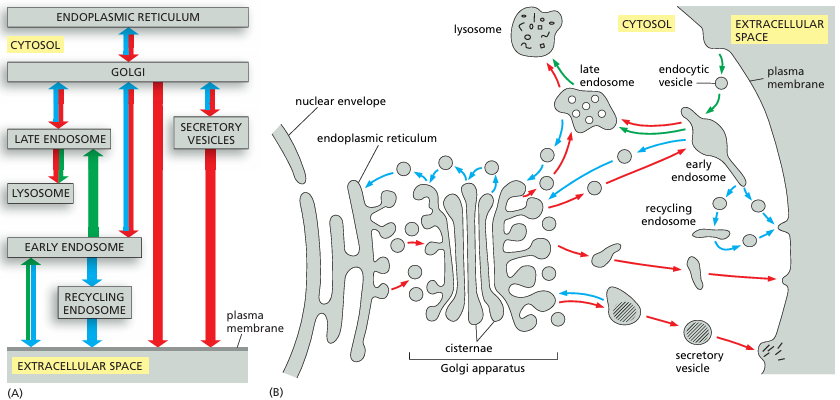
\includegraphics[width=\textwidth]{3}
	\caption{A “road-map” of the secretory and endocytic pathways.}
	\label{roead_map}
\end{figure}

\subsubsection{Vesicle Transport}
Vesicle transport refers to the movement of cargo within cells via membrane-bound carriers. \textbf{Note that vesicles are \underline{not} always spherical}. The movement of vesicles is often aided by the \textbf{cytoskeleton}. For instance vesicles can move along \textbf{microtubules via motor-proteins}. 

\begin{DefWithTitle}{Exocytosis}
	\gls{exocytosis} is a cellular process in which substances contained in vesicles are released from the cell to the extracellular environment by fusion of the vesicle with the plasma membrane. 
\end{DefWithTitle}

\begin{DefWithTitle}{Endocytosis}
	\gls{endocytosis} is a cellular process in which the cell membrane folds inward to form a vesicle that encloses extracellular material for internalization into the cell
\end{DefWithTitle}

\noindent As a \textbf{consequence of vesicular transport}, exocytosis and endocytosis, compartments that are able to communicate and they will be topologically equivalent. 

\begin{DefWithTitle}{Topologically equivalent}
	The concept of \textit{topological equivalence} refers to the idea that membrane leaflets facing the cytosol share a similar composition and can directly communicate with each other. In contrast, the \textbf{luminal spaces of organelles are topologically equivalent to the extracellular space}. This relationship arises as a \textbf{consequence of vesicular transport}, which preserves membrane orientation during budding and fusion.
\end{DefWithTitle}

\begin{figure}[H]
	\centering
	\subfigure[Exocytosis and Endocytosis]{
		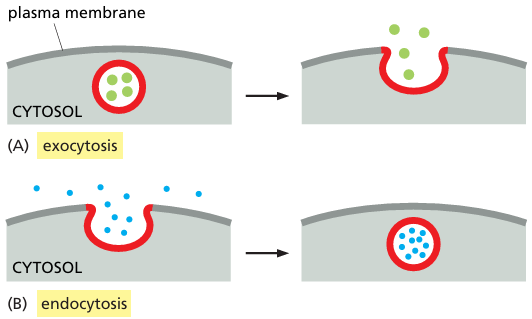
\includegraphics[width = 0.3 \textwidth]{1}
	}
	% Second subfigure
	\subfigure[Vesicle transport]{
		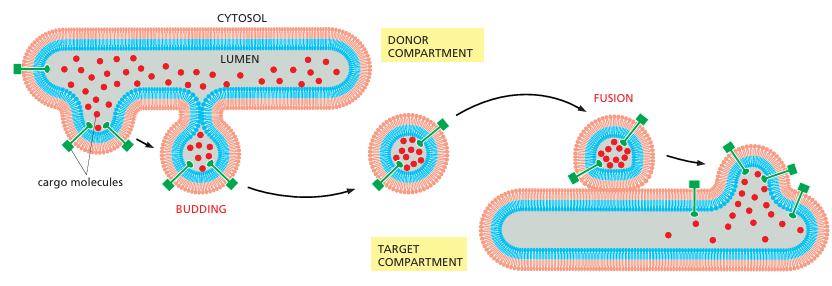
\includegraphics[width = 0.65 \textwidth]{2}
		\label{reactivity}
	}
	\caption{Topologically equivalent compartments, are able to "communicate"}
\end{figure}
\noindent
Most transport vesicles form from specialized, coated regions of membranes . There are \textbf{various types of coated vesicles}, which have distinctive cage of proteins covering their \textbf{cytosolic face}. Before they fuse with the target membrane they \textbf{discard their coat}. This is required for the membranes to fuse. \\
\\
The \textbf{coat} performs two main function: 
\begin{itemize}
	\item The inner layer selects the appropriate membrane molecules for transport.
	\item The outer layer shapes the vesicle.
\end{itemize} 
There are three well-characterized types of coated vesicles, distinguished by their major coat proteins: clathrin-coated, COPI-coated, and COPII-coated. Each type is used for different trasport steps. 

\begin{figure}[H]
	\centering
	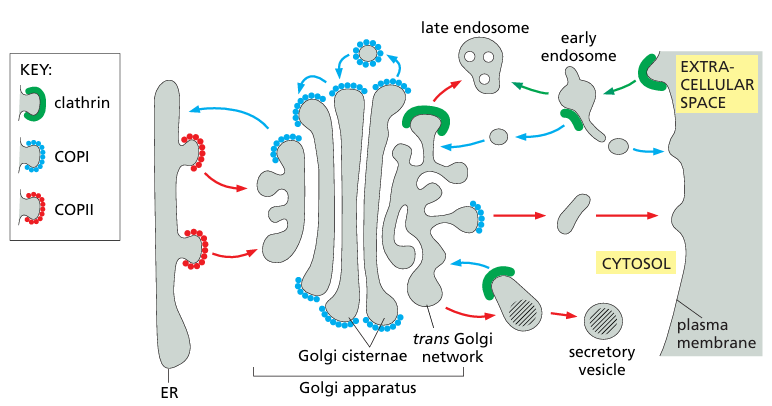
\includegraphics[width=0.65 \textwidth]{5}
	\caption{Use of different coats for different steps in vesicle traffic}
\end{figure}


\paragraph{Clathrin-coated vesicle}
\indent The major protein component of clathrin-coated vesicles is \textbf{\gls{clathrin}} itself, which forms the outer layer of the coat. Each clathrin subunit consists of \textbf{three large and three small polypeptide chains} that together form a three-legged struc ture called a \textbf{triskelion}. These triskelions assemble into a \textbf{basketlike framework} of hexagons and pentagons to form coated pits (\textbf{buds}) on the cytosolic surface of membranes. \\
\\
\indent \textbf{The specificity does not come from the coat but from adapter proteins}. They are a major component and bind the clathrin coat to the membrane and trap various transmembrane proteins - the so called \textbf{cargo receptors}. There are several adapter proteins each is specific for a different set of cargo proteins. 

\begin{figure}[H]
	\centering
	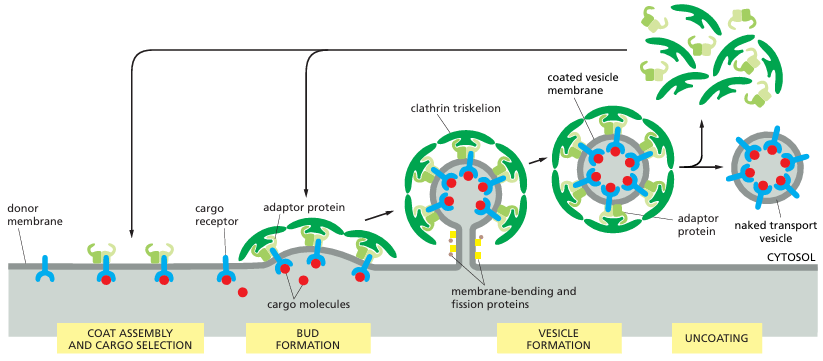
\includegraphics[width= \textwidth]{7}
	\caption{The assembly and disassembly of a clathrin coat}
\end{figure}


\begin{ExWithTitle}{The adaptor protein AP2}
	\gls{AP2} binds to \textbf{specific phosphorylated phosphoinositides} in the plasma membrane, which triggers a conformational change exposing binding sites for cargo receptors. Acting as a \textbf{coincidence detector}, it requires simultaneous interactions with both lipids and cargo to stably associate with the membrane. Upon binding, AP2 induces membrane curvature and promotes clathrin coat assembly, \textbf{facilitating vesicle formation}. See fig. \ref{AP2} 
\end{ExWithTitle}

\begin{RemarkWithTitel}{BAR domains, bending membrane}
	\gls{BARdomain} proteins are diverse and enable many membrane-bending processes in the cell. BAR domains are built from coiled coils that dimerize into modules with a positively charged inner surface, which preferentially interacts with negatively charged lipid head groups \textbf{to bend membranes}. See fig. \ref{BARdomain}  
\end{RemarkWithTitel}

\begin{figure}[H]
	\centering
	\subfigure[Lipid-induced conformation 
	switching of AP2.]{
		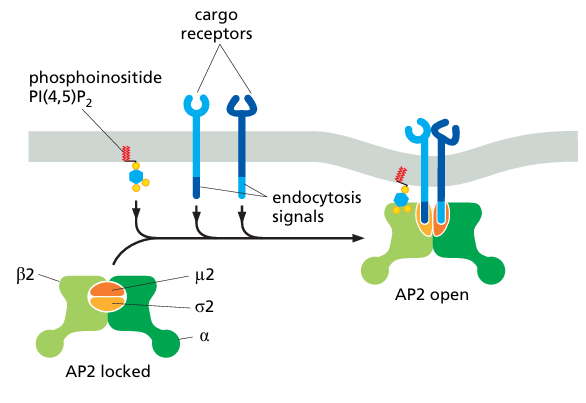
\includegraphics[width = 0.55 \textwidth]{8}
		\label{AP2}
	}
	% Second subfigure
	\subfigure[The structure of BAR domains]{
		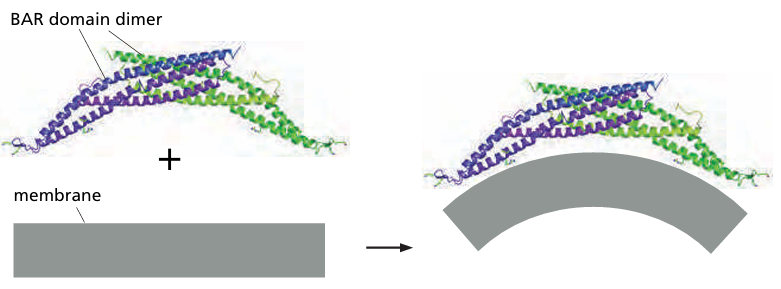
\includegraphics[width = 0.4 \textwidth]{9}
		\label{BARdomain}
	}
	\caption{}
\end{figure}
\noindent
As the bud grows, cytoplasmic proteins, including \textbf{\gls{dynamin}}, assemble at the neck. Dynamin contains a PI(4,5)
P2-binding domain, which tethers the protein to the membrane, and a \textbf{GTPase domain}, which regulates the rate at which vesicles \textbf{pinch of from the membrane}. \\
\indent To bring the two noncytosolic leaflets of the membrane into close proximity in order to fuses them dynamin recruits other proteins helping to bend the patch of membrane.  See fig. \ref{dynamin}

\begin{figure}[H]
	\centering
	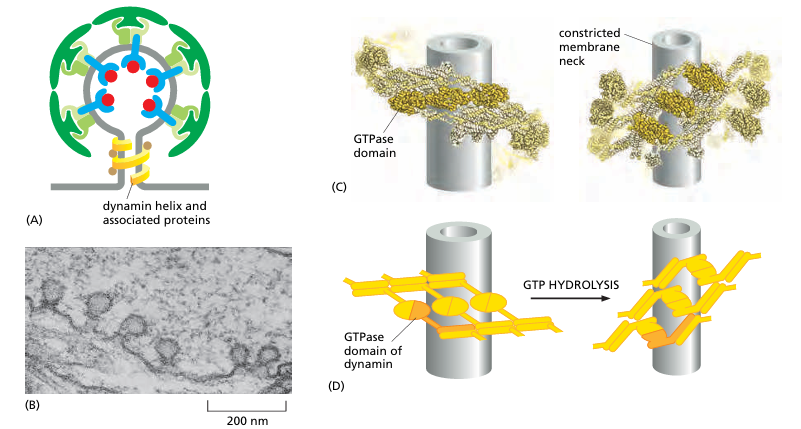
\includegraphics[width=0.8\textwidth]{10}
	\caption{The role of dynamin in pinching off clathrin-coated vesicles.}
	\label{dynamin}
\end{figure}


\paragraph{COPII-coated vesicle}
There are many ways to regulate coat formation. For example \textbf{Coat-recruitment GTPases} control the assembly of clathrin coats on endosomes and the COPI and COPII coats on Golgi and ER membranes.\\
The \textbf{\gls{sar1} protein} responsible for the COPII coats at the ER membrane is part of the Coat-recruitment GTPase family. \\
\\
\textbf{Coat-recruitment GTPases} are usually found in high concentration in the cytosol in an inactive, GDP-bound state. In the formation of a COPII-coated vesicle, \textbf{Sar1-GEF is embedded in the ER} membrane and binds to the \textbf{cytosolic Sar1}, causing Sar1 to \textbf{release GDP and bind GTP}. This leads to the \textbf{expression an amphiphilic helix}, which inserts into the cytoplasmic leaflet of the lipid bilayer. Sar1 then \textbf{recruits} adaptor coat protein (like \textbf{\gls{sec23}} and \textbf{\gls{sec24}}) subunits to \textbf{initiate budding}. See fig. \ref{COPII}

\begin{figure}[H]
	\centering
	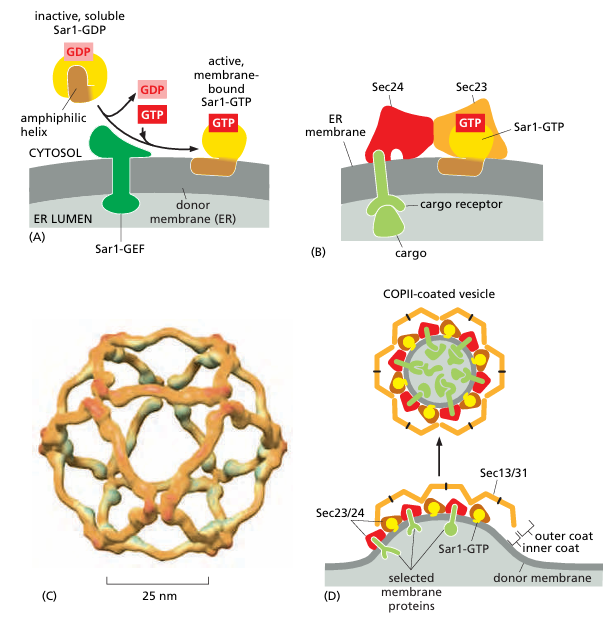
\includegraphics[width=0.7\textwidth]{11}
	\caption{Formation of a COPII coated vesicle.}
	\label{COPII}
\end{figure}


\subsubsection{Recognizion of Destination}
Specificity in targeting is ensured because all transport vesicles display surface markers that identify them according to their origin and type of cargo. Moreover target membrane displays complementary receptors that recognize this markers. \\
\\
First, \textbf{Rab proteins} and Rab effectors direct vesicles to specific spots on the correct target membrane. In addition, distinct \textbf{phosphoinositide compositions} on different membranes help recruit the correct Rab effectors, adaptors, and SNARE regulators to ensure fidelity. Second, \textbf{SNARE proteins} and SNARE regulators mediate the fusion of the lipid bilayers.

\begin{RemarkWithTitel}{PIPs varies from organelle to organelle}
	Recall that PIPs varies from organelle to organelle. Many proteins involved in vesicle transport contain domains that bind with high specificity to the head group of particular PIPs. Therefore local control of the PI and PIP kinases and PIP phosphatases is important for the control of the vesicle traffic. See fig. \ref{PIPloc} 
\end{RemarkWithTitel}

\begin{figure}[H]
	\centering
	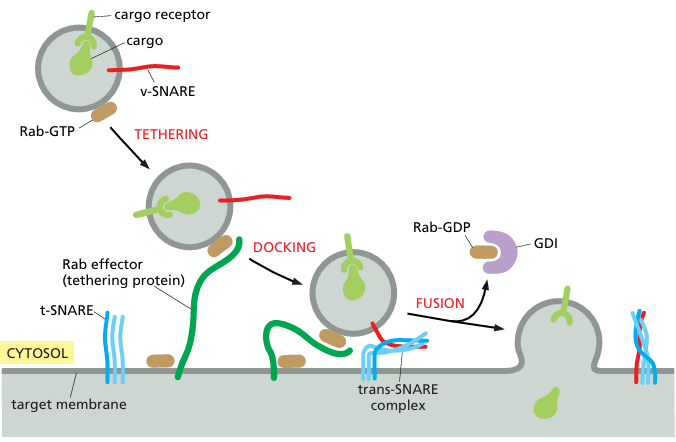
\includegraphics[width=0.7\textwidth]{13}
	\caption{Tethering of a transport vesicle to a target membrane.}
\end{figure}


\paragraph{Rab proteins}

\gls{Rab} is a family of small GTPases that regulate vesicle transport by ensuring specificity in vesicle targeting. Rab proteins recruit effector molecules that help guide vesicles to the correct membrane compartment. \\
\\
\textbf{Like coat-recruitment GTPases}, Rab proteins cycle between a membrane and the cytosol. In their GDP-state they are in they cytosol bound to an other protein that keeps them soluble. While in the \textbf{GTP-state} they are active and tightly associated with the membrane transport. \\
\\
\textbf{Membrane bound Rab-GEFs} activate Rab proteins on both transport vesicles and target membranes. Once in the \textbf{GTP-state they bind} to other proteins called, \textbf{Rab effectors}, which are the downstream mediators of vesicle transport. 

\begin{figure}[H]
	\centering
	\subfigure[Subcellular Locations of Some Rab Proteins]{
		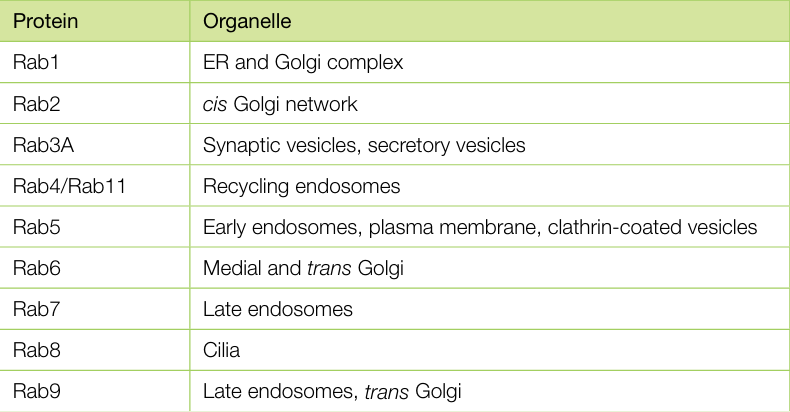
\includegraphics[width = 0.5 \textwidth]{16}
	}
	% Second subfigure
	\subfigure[A model for a generic Rab cascade.]{
		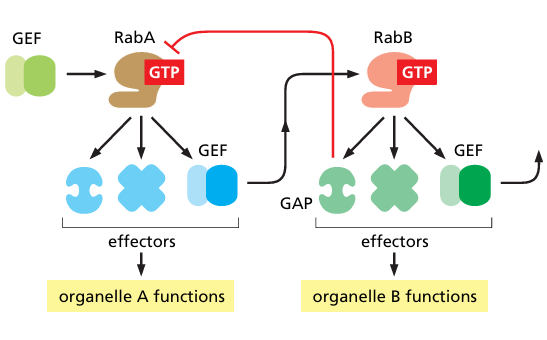
\includegraphics[width = 0.45 \textwidth]{15}
		\label{RABcascade}
	}
	\caption{Rab}
\end{figure}

The assembly of Rab proteins and their effectors on a membrane is cooperative and results in the formation of large, \textbf{specialized membrane patches. Rab5}, for example, assembles on e\textbf{ndosomes and mediates the capture of endocytic vesicles} arriving from the plasma membrane.

\begin{figure}[H]
	\centering
	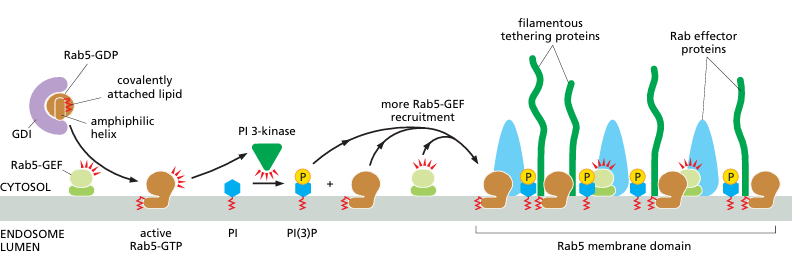
\includegraphics[width=0.8\textwidth]{17}
	\caption{The formation of a Rab5 domain on the endosome membrane.}
\end{figure}

A Rab domain can be disassembled and \textbf{replaced by a different Rab} domain, changing the identity of an organelle. Such ordered recruitment of sequentially acting Rab proteins is called a \textbf{Rab cascade}. See fig. \ref{RABcascade} \\
Over time, for example, \textbf{Rab5 domains are replaced by Rab7} domains on endosomal membranes. This converts an \textbf{early endosome}, marked by Rab5, into a \textbf{late endosome}, marked by Rab7.

\paragraph{SNARE proteins}

\textbf{Membrane fusion} requires bringing the lipid bilayers of two membranes to within \textbf{1.5 nm} of each other so that they can merge. When 
the membranes are in such close apposition, lipids can flow from one bilayer to the other. \\
\\
For this close approach, \textbf{water must be displaced} from the hydrophilic surface of the membrane—a process that is highly energetically unfavorable and requires \textbf{specialized fusion proteins} that overcome this energy barrier.\\
\\
\gls{SNARE} are a group of membrane-associated proteins that mediate the fusion of vesicle and target membranes. SNAREs on the vesicle (v-SNAREs) and on the target membrane (t-SNAREs) form complexes that bring membranes close enough to fuse. \\
Note that SNARE complexes can only be made with certain combinations and thus define \textbf{specificity}. \\
\\
In addition to the specificity of t- and v-SNARES, \textbf{Rab proteins can regulate the availability of SNARE} proteins. 

\begin{figure}[H]
	\centering
	\subfigure[The intracellular location of phosphoinositides.]{
		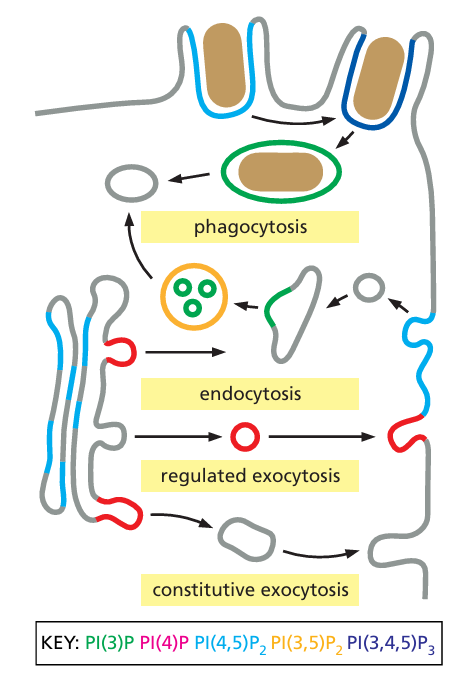
\includegraphics[width = 0.4 \textwidth]{6}
		\label{PIPloc}
	}
	% Second subfigure
	\subfigure[SNARE proteins may catalyze membrane fusion]{
		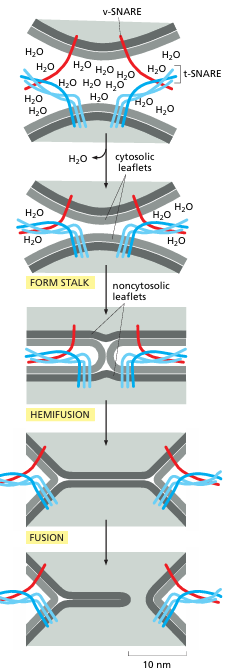
\includegraphics[width = 0.2 \textwidth]{12}
		\label{SNARE}
	}
	\caption{}
\end{figure}

\textbf{Intacting SNAREs need to be pried apart before they can function again}. A crutial protein to archive this is \textbf{\gls{NSF}}, an ATPase that disassembles SNARE complexes after membrane fusion. \textbf{NSF uses energy} from ATP hydrolysis to recycle SNARE proteins for further rounds of vesicle fusion. This is because the SNARE Complex is just that damn stable.\\
\\  
Note the requirement for NSF-mediated reactivation of SNAREs by SNARE complex disassembly helps prevent membranes from fusing indiscriminately. NSF can be used to activate the SNARE machinery at the right time.   
\begin{figure}[H]
	\centering
	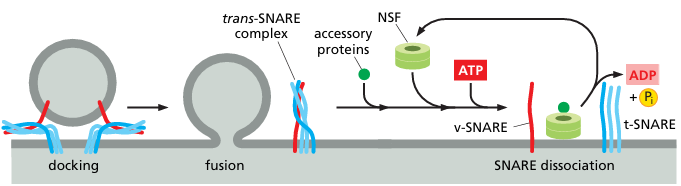
\includegraphics[width=0.8\textwidth]{14}
	\caption{Dissociation of SNARE pairs by NSF after a membrane fusion cycle.}
\end{figure}
	
	
\subsection{Between ER and Golgi}
The newly synthesized proteins cross the \textbf{ER} membrane from the \textbf{cytosol} to enter the \textbf{secretory pathway}. Then they will get transported from the \textbf{ER to the Golgi apparatus} and from there to the \textbf{cell surface}. The proteins are \textbf{successively modified} as they pass through a series of compartments. \\
\\ 
Recall that the \textbf{Glogi apparatus} is a major site of carbohydrate synthesis, as well as a sorting and dispatching station for products from the ER. \\
\\
Proteins that have entered the ER ans are destined for the Golgi apparatus or beyond are first packed into \textbf{COPII-coated} trasnport vesicles. These vesicles bud from specialized regions of the ER called \textbf{ER exit sites}, whose membrane lacks bound ribosomes. The cargo membrane proteins display exit signlas on their cytosolic surface that adaptor proteins of the inner COPII coat recognize. \textit{Note some of theses cargo proteins will be recycled back to the ER once they have delivered their cargo.} \\
\\
Moreover the transport from the ER to the Golgi appartus serves also as a \textbf{quality control step}. Then to  exit from the ER, proteins must be \textbf{properly folded} and, if they are subunits of multiprotein complexes, they need to be \textbf{completely assembled}. Those that are misfolded or incompletely assembled transiently remain in the ER, where they are bound to chaperone proteins. 

\begin{DefWithTitle}{Homotypic membrane fusion}
		After transport vesicles have budded from ER exit sites and have shed their coat, they begin to \textbf{fuse with one another}. This is called \gls{homotypicfusion}, in contrast to heterotypic fusion where compartments from different origin fuse. For \gls{homotypicfusion} \textbf{matching SNAREs} are required.	
\end{DefWithTitle}
When ER-derived vesicles fuse with one another we speak of \textbf{\gls{VTC}}. These are generated continuously and makes the transport more efficient as: They send transport vesicles on their own (\textbf{COPI-coated}) that feed into the \textbf{retrievel pathway}; They move quickly along \textbf{microtubules} (using \textbf{motor proteins}) from the ER to the Golgi. 

\begin{figure}[H]
	\centering
	\subfigure[Homotypic membrane fusion.]{
		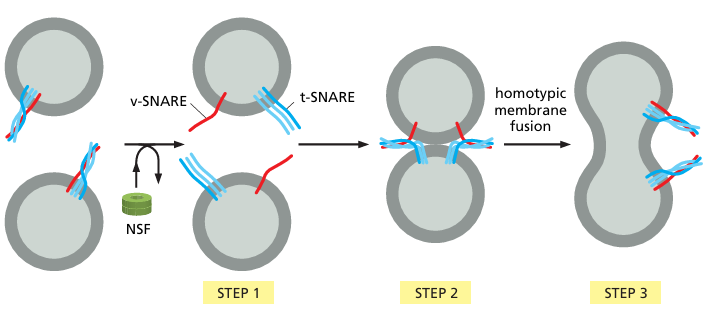
\includegraphics[width = 0.6 \textwidth]{18}
		\label{Homotypic_membrane}
	}
	% Second subfigure
	\subfigure[Vesicular tubular clusters.]{
		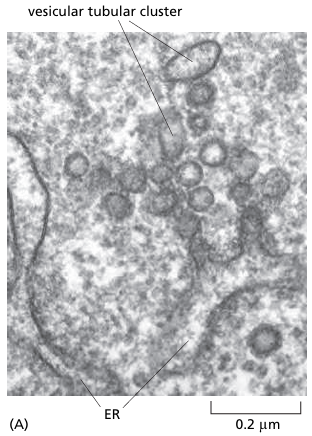
\includegraphics[width = 0.2\textwidth]{19}
	}
	\caption{Vesicular Tubular Clusters Mediate Transport from the ER to the Golgi Apparatus }
\end{figure}

Since \textbf{Biology is imperfect} sometimes a soluble \textbf{ER resident protein is wrongfully imported} to the Golgi. This creates the need of a \textbf{backward (retrieval) transport}. \\
\\
This transport is mediated by \textbf{COPI-coated} vesicles. Therefore resident ER membrane proteins contain signals that directly bind to COPI coats. The best-characterized retrieval signal of this type is the \textbf{\gls{kkxx}} (Lysine-Lysine-X-X). \\
\\
However, \textbf{soluble ER resident proteins}, such as BiP, also contain a short ER retrieval signal at their C-terminal end: it consists of a Lys-Asp-Glu-Leu or a similar sequence. This signal is called \textbf{\gls{KDEL}}. Note that if this signal is removed from BiP by genetic engineering, the protein is slowly secreted from the cell. \\
\indent These proteins then bind to the \textbf{KDEL receptor} a multipass transmembrane protein, which cycles between the ER and Golgi. Therefore the receptor must have a different affinity for the KDEL sequence depending on its location. This can be explained by the \textbf{lower pH in the Golgi compartments}. 

\begin{figure}[H]
	\centering
	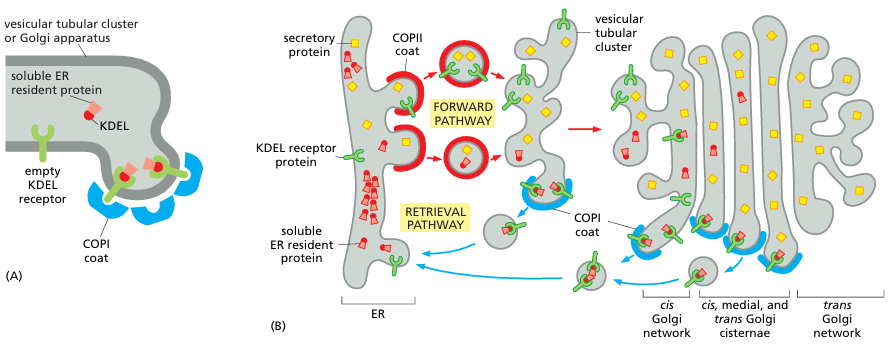
\includegraphics[width= \textwidth]{20}
	\caption{Retrieval of soluble ER resident proteins.}
\end{figure}

\begin{RemarkWithTitel}{Kin Recognition}
	Not all proteins with a KDEL signal are efficiently retained in the ER. This suggests that, beyond KDEL-based retrieval, \textit{\gls{kinrecognition}} may contribute to ER retention. ER-resident proteins may interact with one another, slowing their export. Thus, proteins lacking KDEL but interacting with ER residents are still retained longer than typical secreted proteins.
\end{RemarkWithTitel}

\subsection{In the Golgi Appartus}
Each Golgi stack typically \textbf{consists of four to six cisternae}. Tubular connections between corresponding cisternae link many stacks, thus forming a single complex, which is usually located \textbf{near the cell nucleus and close to the centrosome}. \textit{Note its localization depends on microtubules. If microtubules are experimentally depolymerized, the Golgi apparatus reorganizes into individual stacks that are found throughout the cytoplasm, adjacent to ER exit sites.} \\
\indent There are \textbf{two possible models} explaining the movement through the Golgi. However it is likely that the \textbf{truth lies somewhere in between}. A long-lasting cisternae might exist in the center of each Golgi cisterna, while regions at the rim may undergo continuous maturation, perhaps utilizing Rab cascades that change their identity.
\begin{figure}[H]
	\centering
	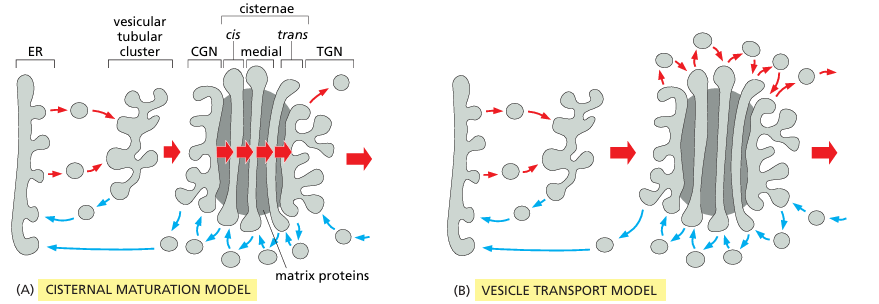
\includegraphics[width= 0.9 \textwidth]{26}
	\caption{Two possible models explaining the organization of the Golgi and how proteins move through it.}
\end{figure}

\begin{RemarkWithTitel}{Golgi Matrix Proteins Help Organize the Stack}
	The distinctive structure of the Golgi apparatus relies apart from both the microtubule cytoskeleton also on a \textbf{network of Golgi matrix proteins}. These matrix proteins form a \textbf{scaffold between adjacent cisternae}, helping maintain the Golgi stack’s architecture. Among them, \textbf{golgins} play a key role. Golgins are long, coiled-coil proteins with flexible hinge regions that \textbf{extend like tentacles}—up to 100–400 nm from the Golgi surface. They help c\textbf{apture and retain transport vesicles} near the Golgi by \textbf{interacting with Rab proteins}, thus supporting efficient vesicle docking and trafficking. See \textbf{fig. \ref{golgins}}
\end{RemarkWithTitel}

\begin{figure}[H]
	\centering
	\subfigure[Oligosaccharide processing in Golgi compartments]{
		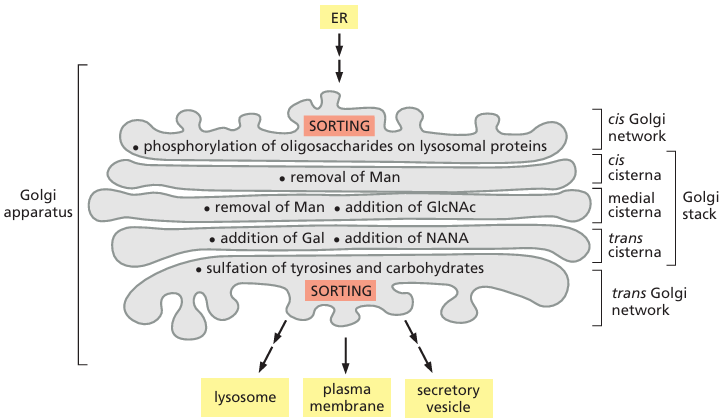
\includegraphics[width = 0.6\textwidth]{21}
	}
	% Second subfigure
	\subfigure[A model of golgin function]{
		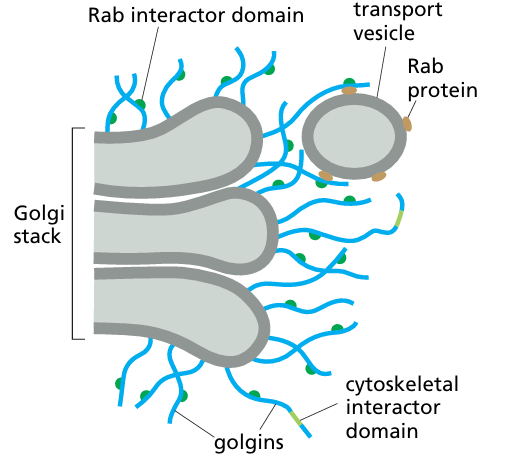
\includegraphics[width = 0.35\textwidth]{27}
		\label{golgins}
	}
	\caption{Oligosaccharide Chains Are Processed in the Golgi Apparatus}
\end{figure}

Note that during their passage through the Golgi (\textbf{cis face} (or entry face) to \textbf{trans face} (or exit face)), transported molecules undergo an ordered \textbf{series of modification}.

\subsubsection{Glycosylation in the Golgi}
Whereas the ER lumen is full of soluble lumenal resident proteins and enzymes, the \textbf{resident proteins in the Golgi apparatus are all membrane bound}. Therefore the enzymatic reactions occur entirely on the membrane surface. For example Golgi glycosidases and glycosyl transferases are single-pass transmembrane proteins, many of which are organized in multienzyme complexes.\\
\\
Two broad classes of \textbf{N-linked oligosaccharides}, the complex oligosaccharides and the high-mannose oligosaccharides, are attached to mammalian glycoproteins. \textit{Sometimes, both types are attached (in different places) to the same polypeptide chain.} 
\begin{itemize}
	\item \textbf{Complex oligosaccharides} are generated when the original N-linked oligosaccharide added in the ER is trimmed and further sugars are added.
	\item By contrast, \textbf{high-mannose oligosaccharides} are trimmed but have no new sugars added to them in the Golgi apparatus.
\end{itemize}

Whether a given oligosaccharide remains high-mannose or is processed depends largely on its position in the protein. If the oligosaccharide is accessible to the processing enzymes in the Golgi apparatus, it is likely to be converted to a complex form. 

\begin{RemarkWithTitel}{Endo H} 
	\gls{EndoH}  is short  for Endoglycosidase H, an enzyme that cleaves high-mannose and some hybrid N-linked oligosaccharides from glycoproteins (\textbf{Endo H-sensitive}). It does not cleave complex oligosaccharides (\textbf{Endo H-resistant}), making it a useful tool to distinguish between early (ER) and later (Golgi-processed) stages of glycan maturation.
\end{RemarkWithTitel}
Note that \textbf{sialic acids} is of special relevance as it has a \textbf{negative charge}.

\begin{figure}[H]
	\centering
	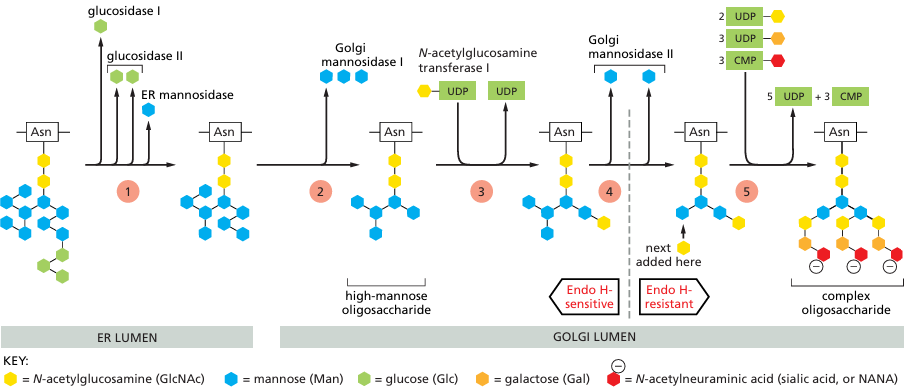
\includegraphics[width= \textwidth]{23}
	\caption{Oligosaccharide processing in the ER and the Golgi apparatus.}
\end{figure}

In addition there are also some proteins that have sugars added to hydroxyl groups of selected serines or theronines. These are \textbf{O-linked glycosylations} and like N-linked they are catalyzed by a series of glycosyl transferase enzymes that use sugar nucleotides in the lumen of the Golgi. Therefore the Golgi produces \textbf{mucins} (heavily glycosylated proteins found in mucus) and \textbf{Proteoglycans} (proteins with one or more glycosaminoglycan (GAG) chains). \\
\\
Moreover sugars in \textbf{\gls{GAGs} are heavily sulfated in the Golgi} apparatus right after the polymers are synthesized. This sulfation contributes significantly to their strong negative charge. In addition, some tyrosine residues in proteins are also sulfated just before the proteins leave the Golgi. In both cases, \textbf{the sulfate groups are donated by \gls{PAPS}}.

\begin{figure}[H]
	\centering
	\subfigure[N- and O-linked glycosylation]{
		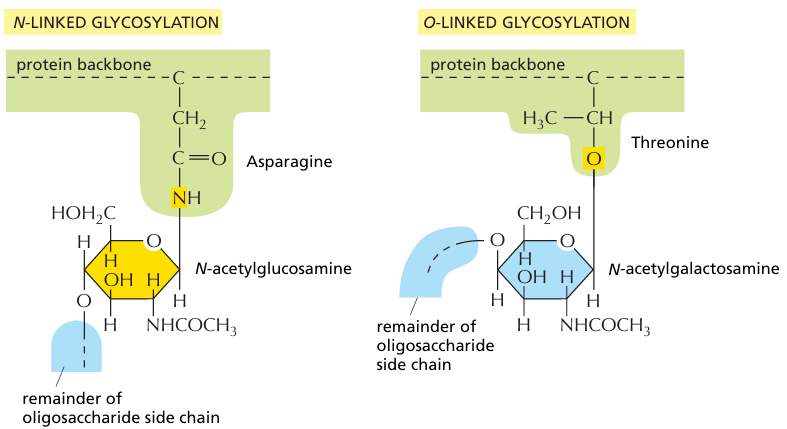
\includegraphics[width = 0.55\textwidth]{24}
	}
	% Second subfigure
	\subfigure[The structure of PAPS]{
		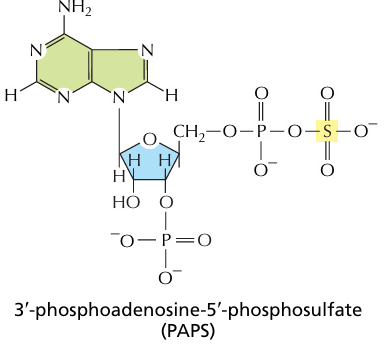
\includegraphics[width = 0.3\textwidth]{25}
	}
	\caption{Proteoglycans Are Assembled in the Golgi Apparatus}
\end{figure}

\begin{DefWithTitle}{Lectins}
		\gls{lectin}s are a type of protein that specifically binds to carbohydrate structures without modifying them. Therefore, it plays key roles in cell–cell recognition, signaling, and intracellular trafficking by recognizing specific glycan patterns on glycoproteins and glycolipids. In the Golgi apparatus and elsewhere, lectins help sort glycoproteins by interacting with their attached sugar chains. 
\end{DefWithTitle}

\begin{RemarkWithTitel}{Purpose of glycosylation}
	The purpose of glycosylation is diverse: 
	\begin{itemize}
		\item  \textbf{N-linked glycosylation promotes protein folding} in two ways. First, it has a direct role in making folding intermediates \textbf{more soluble}, thereby preventing their aggregation. Second, the sequential modifications of the N-linked oligosaccharide establish a \textbf{“glyco-code” that marks the progression} of protein folding and mediates the binding of the protein to chaperones. 
		\item It \textbf{protects proteins} protruding the surface, thus limiting the approach of other macromulecules, like proteolytic enzymes. 
		\item The mucus coat of lung and intestinal cells \textbf{protects against many pathogens}.
		\item The recognition of sugar chains by lectins in the extracellular space is important in many developmental processes and in \textbf{cell–cell recognition}. 
		\item Glycosylation can also have important \textbf{regulatory roles}. For example Notch where glycosylation changes the specificity. 
	\end{itemize}
\end{RemarkWithTitel}

\subsection{Around Lysosomes}

Lysosomes are membrane-enclosed organelles filled with soluble hydrolytic enzymes that digest macromolecules. Theses enzymes are \textbf{acid hydrolases}; that are hydralases that work at acidic pH. Therefore theses enzymes do  not work outside of the lysosome, otherwise it would be pretty dangerous if those enzymes would go berserk. To maintain the low pH lysosomes uses a vocuolar H+ ATPase (V-type ATPase). \\
\\
\textbf{Lysosomes are a meeting place} where seeveral streams of intracellular traffic converge. A route that leads outward from the ER via the Golgi apparatus delivers most of the lysosome’s digestive enzymes, while at least \textbf{four paths} from different sources feed substances into lysosomes for digestion: 
\begin{itemize}
	\item \textbf{Endocytosis} – internalizes molecules from the extracellular fluid into the cell.
	\item \textbf{Phagocytosis} – specialized in engulfing large particles or microorganisms, mainly by immune cells.
	\item \textbf{Macropinocytosis} – non-specifically engulfs extracellular fluid, membrane, and surface-bound particles.
	\item \textbf{Autophagy} – degrades cytosolic components and damaged organelles from within the cell.
\end{itemize}

\paragraph{Lysosome Maturation}
Lysosome maturation is a dynamic, multistep process that transforms \textbf{late endosomes into fully functional lysosomes}. This maturation involves:
\begin{itemize}
	\item \textbf{Fusion of late endosomes} with existing lysosomes and vesicles from the Golgi, which deliver newly synthesized acid hydrolases.
	\item \textbf{Formation of endolysosomes}, hybrid compartments where active degradation begins.
	\item As contents are digested, the endolysosome \textbf{condenses and matures into a “classical” lysosome} — dense and enzyme-rich.
	\item \textbf{Mature lysosomes can re-enter the cycle}, fusing with other endosomes or endolysosomes to continue degradation.
\end{itemize}
Because of this continuous remodeling, lysosomes appear \textbf{morphologically diverse} and are better understood as \textit{stages of a maturation cycle}, not fixed entities.

\begin{figure}[H]
	\centering
	\subfigure[Four pathways to degradation in lysosomes.]{
		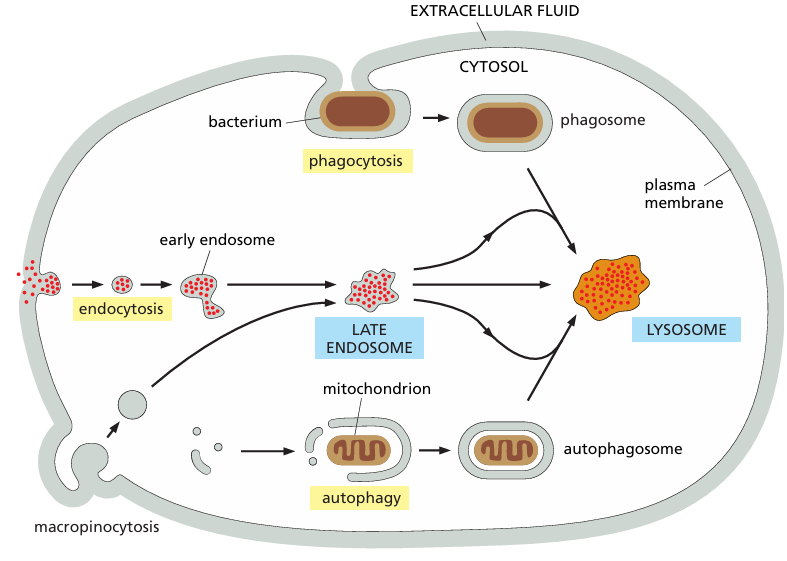
\includegraphics[width = 0.5\textwidth]{28}
	}
	% Second subfigure
	\subfigure[A model for lysosome maturation.]{
		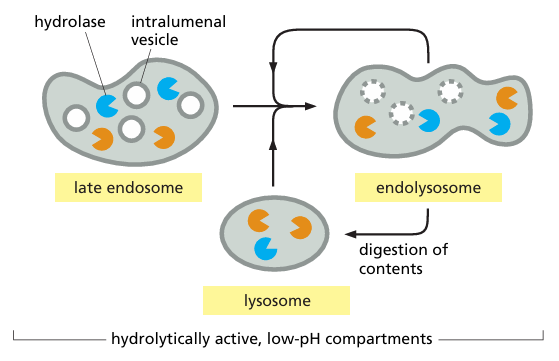
\includegraphics[width = 0.4\textwidth]{29}
	}
	\caption{Lysosomes Are Heterogeneous}
\end{figure}

\begin{RemarkWithTitel}{ Autophagy Degrades Unwanted Proteins and Organelles}
	When a signaling pathway is activated, it triggers the start of autophagosome formation in the cytoplasm. A curved membrane structure begins to grow, formed by the fusion of small vesicles from unknown sources. This eventually closes into a double membrane, creating an autophagosome that surrounds part of the cytoplasm. The autophagosome then fuses with lysosomes, where the enclosed material is broken down by digestive enzymes. During this process, special ubiquitin-like proteins are activated by attaching to lipid anchors, helping to shape the membrane and guide vesicle fusion.
\end{RemarkWithTitel}

\begin{figure}[H]
	\centering
	\subfigure[A crescent of autophagosomal membrane grows by fusion of vesicles of unknown origin]{
		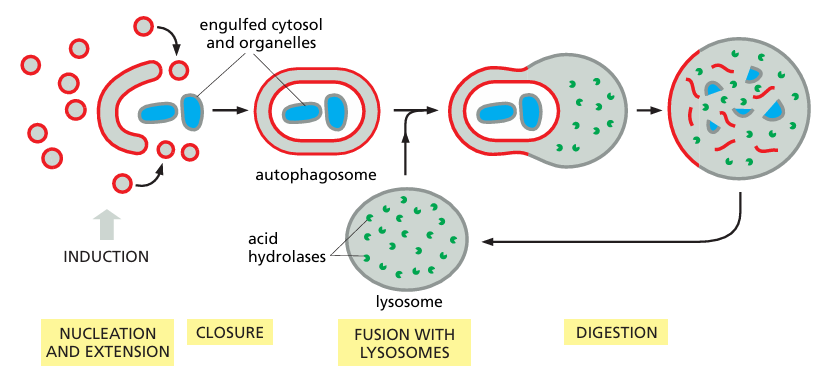
\includegraphics[width = 0.7\textwidth]{33}
	}
	% Second subfigure
	\subfigure[An electron micrograph]{
		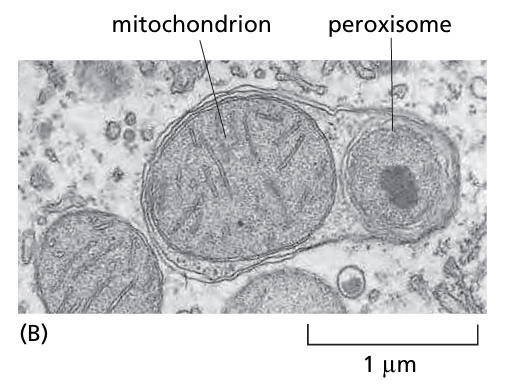
\includegraphics[width = 0.2\textwidth]{34}
	}
	\caption{A model of autophagy}
\end{figure}

\paragraph{Delivery of lysosomal hydrolases from the TGN to the lysosome}
The enzymes are first delivered to endosomes in transport vesicles that 
bud from the TGN (trans golgi network), before they move on to endolysosomes and lysosomes (maturation of Lysosomes). \\
\\
Lysosomal hydrolases are \textbf{recognized} and selected in the TGN because of a unique marker. \textbf{Mannose 6-phosphate (\gls{m6p})} groups are added exclusively to the \textbf{N-linked oligosaccharides} of these soluble lysosomal enzymes as they pass through the lumen of the cis Golgi network. \\
\indent Transmembrane \textbf{M6P receptor proteins}, which are present in the TGN, recognize the M6P groups and bind to the lysosomal hydrolases on the lumenal side of the membrane and to adaptor proteins in assembling \textbf{clathrin coats} on the cytosolic side. In this way, the receptors help package the hydrolases into clathrin-coated vesicles that bud from the TGN and deliver their contents to early endosomes.\\
\\
The M6P receptor (like many proteins in transport) is an example for a protein that \textbf{changes specificity}: The M6P receptor protein binds to M6P at pH 6.5–6.7 in the TGN lumen and releases it at pH 6, which is the pH in the lumen of endosomes. 

\begin{figure}[H]
	\centering
	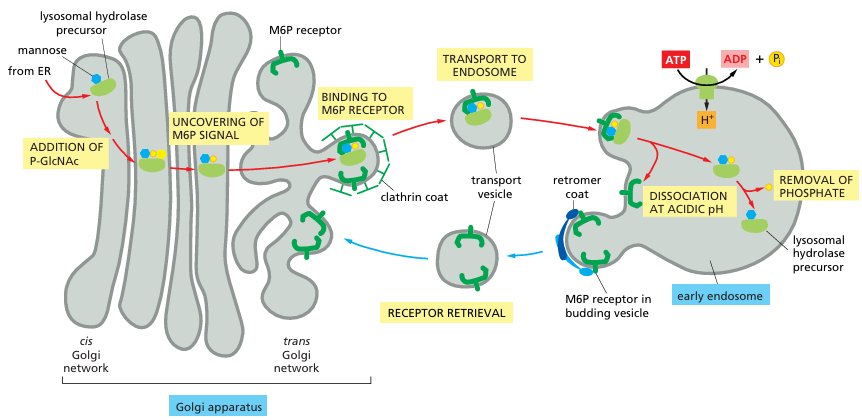
\includegraphics[width= 0.8\textwidth]{31}
	\caption{The transport of newly synthesized lysosomal hydrolases to endosomes.}
\end{figure}

The specialized enzyme called \textbf{GlcNAc phosphotransferase identifies lysosomal hydrolases by recognizing a unique signal patch} on their surface. This enzyme has two distinct domains: a \textbf{recognition site} that binds specifically to the signal patch on lysosomal enzymes, and a \textbf{catalytic site} that attaches a GlcNAc-phosphate group from UDP-GlcNAc to a mannose residue on the hydrolase’s high-mannose N-linked oligosaccharide. Afterward, a second enzyme removes the GlcNAc, leaving behind an exposed \textbf{mannose 6-phosphate} (M6P) the crucial signal for lysosomal targeting.

\begin{figure}[H]
	\centering
	\subfigure[The recognition of a lysosomal hydrolase.]{
		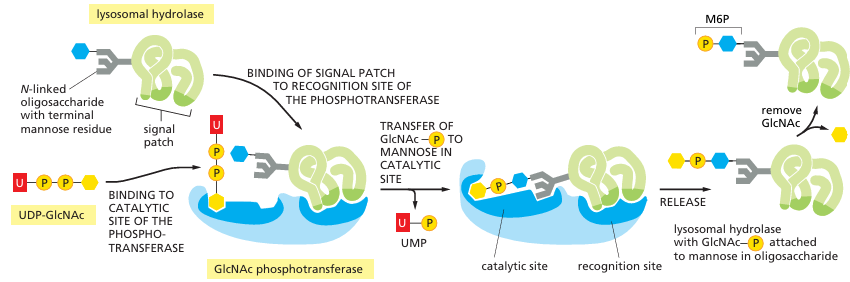
\includegraphics[width = 0.7\textwidth]{32}
	}
	% Second subfigure
	\subfigure[M6P on hydrolase]{
		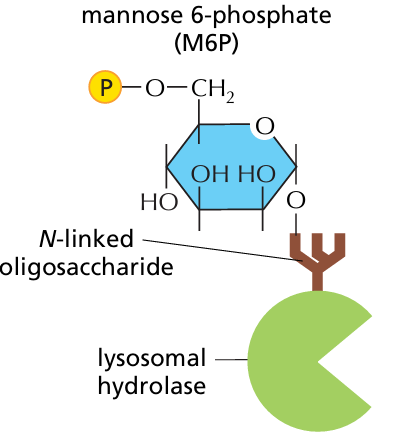
\includegraphics[width = 0.2\textwidth]{30}
	}
	\caption{How are lysosomal hydrolases recognized in the trans golgi network?}
\end{figure}

\subsection{Endocytosis}
The inward routes from the cell surface begin with endocytosis, a process by which cells internalize plasma membrane components, fluids, solutes, macromolecules, and particles. This mechanism allows the cell to dynamically regulate the composition of its plasma membrane in response to changing extracellular conditions.\\
\\
In endocytosis, material is enclosed by an invaginating section of the plasma membrane, which pinches off to form a \textbf{endocytic vesicle} containing the ingested substance. This vesicles are formed constantly in a process called \textbf{\gls{pinocytosis}} ("cell drinking"). Recall that some specialized cells contain dedicated pathways to take up large particles on demand via the process called phagacytosis ("cell eating"). \\
\\
Once generated at the plasma membrane, most endocytic vesicles fuse with a common receiving compartment, the \textbf{early endosome, where internalized cargo is sorted}: some cargo will be \textbf{returned} either directly or via a \textbf{recycling endosome}, and others are designated for degradation by inclusion in a \textbf{late endosome} (Recall endosome maturation). \\
\\
Each of the stages of the endosome maturation (from the early endosome to the endolysosome) is connected through \textbf{bidirectional vesicle transport to the TGN}. This allows for the \textbf{insertion} of newly synthesized materials, such as lysosomal enzymes, and the \textbf{retrieval} of components such as the M6P receptors. 

\begin{figure}[H]
	\centering
	\subfigure[Endosome maturation: the endocytic pathway from the plasma membrane to lysosomes.]{
		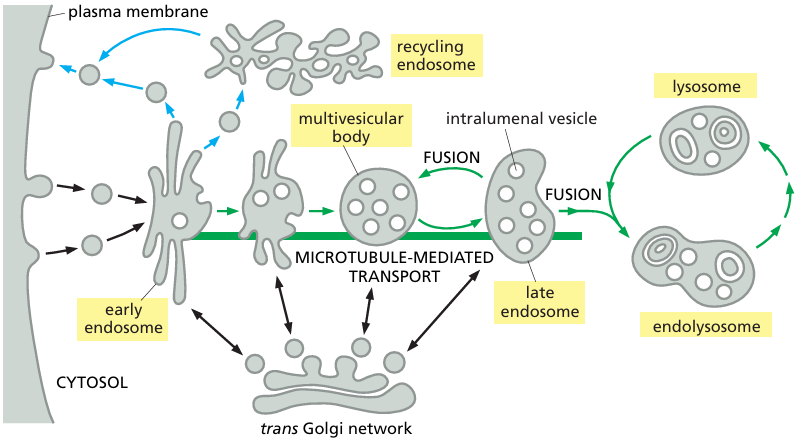
\includegraphics[width = 0.7\textwidth]{35}
	}
	% Second subfigure
	\subfigure[Endocytosis Pathways]{
		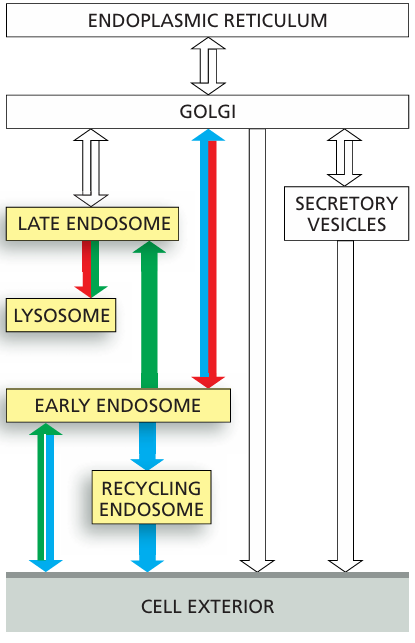
\includegraphics[width = 0.25\textwidth]{36}
	}
	\caption{Transport into the Cell from the Plasma Membrane: Endocytosis}
\end{figure}

The endocytic part of the cycle often begins at \textbf{clathrin-coated pits}. These specialized regions typically occupy about 2 \% of the total plasma membrane area. Note the lifetime of a clathrin-coated pit is short: within a minute or so of being formed, it invaginates into the cell and pinches o to form a clathrin-coated vesicle. \\
\\
In addation to clathrin-coated pits and vesicles, cells can form other types of pinocytic vesicles, such as \textbf{\gls{caveola}}. In contrast to clathrin-coated and COPI- or COPII-coated vesicles, \textbf{caveolae are usually static structures}. They are invagination that form from \textbf{lipid rafts} at the cell surface and bud of to form a \textbf{pinocytic vesicle}. \\
\indent A huge family of structural proteins in caveolae is \textbf{\gls{caveolin}} which cross the membrane extend multiple hydrophobic loops into the membrane from the cytosolic side, but do not cross the the membrane.\\
\\
Moreover, the \textbf{clathrin-coated pits allow for \gls{receptor-mediated-endocytosis}} which is a highly efficient way for cells to take up specific molecules. These molecules (ligands) bind to matching receptors on the cell surface, which cluster into clathrin-coated pits. This process allows cells to concentrate and import even rare substances, \textbf{like cholesterol}, very effectively.

\begin{ExWithTitle}{Colesterol Receptor-Mediated Endocytosis}
	Most cholesterol is transported in the blood as cholesteryl esters in the form of 
	lipid–protein particles known as \textbf{\gls{LDL}}. Therefore a cell can control the import of cholesterol by expressing more transmembrane receptor proteins for LDL. These recpetors are found in clathrin-coated pits and will induce an endocytosis signal.\\
	\indent Moreover, if you think about what colesterol does if this uptake does not work and it accumulates in the blood, it is not surprising that, it was a study of humans with a strong genetic predisposition for atherosclerosis that first revealed the mechanism of receptor-mediated endocytosis.
\end{ExWithTitle}

\begin{figure}[H]
	\centering
	\subfigure[The receptor-mediated endocytosis of LDL.]{
		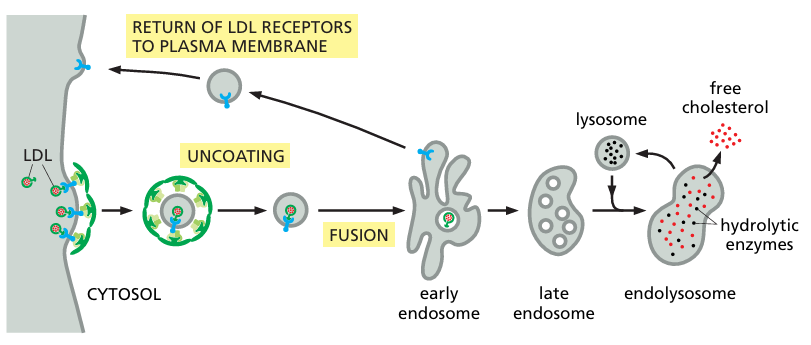
\includegraphics[width = 0.7\textwidth]{38}
	}
	% Second subfigure
	\subfigure[LDL particle]{
		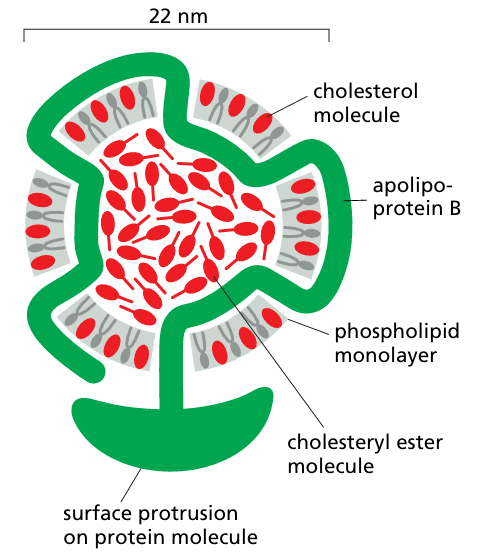
\includegraphics[width = 0.25\textwidth]{39}
	}
	\caption{Receptor-Mediated Endocytosis to Import Selected Extracellula Macromolecules}
\end{figure}

\begin{RemarkWithTitel}{Macropinocytosis}
	\gls{macropinocytosis} is a \textbf{dedicated degradive pathway}. It is also a \textbf{clathrin-independent} endocytic mechanism that can be activated in practically all animal cells. Mostly it does not operate continuously but is rather \textbf{induced for a limited time in response to a cell-surface receptor} activation by a specific cargo (i.e. growth factors). The activation of the rector leads to a complex signaling pathway, resulting in a \textbf{change in actin dynamics} and the \textbf{formation of ruffles} (cell-surface protrusions). When the \textbf{ruffel collapses back onto the cell, the macropinosome is created}. See\textbf{ fig \ref{macropinocytosis}}
\end{RemarkWithTitel}

\begin{figure}[H]
	\centering
	\subfigure[Schematic representation of macropinocytosis.]{
		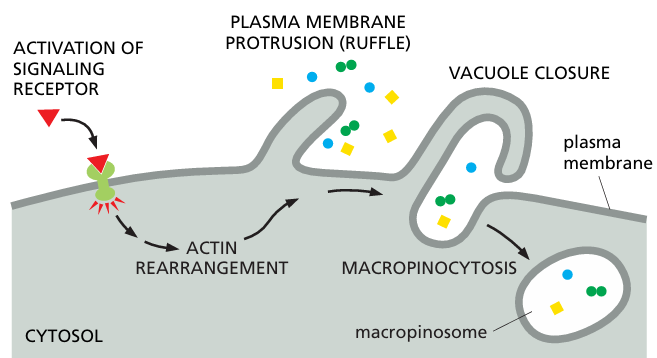
\includegraphics[width = 0.55\textwidth]{37}
		\label{macropinocytosis}
	}
	% Second subfigure
	\subfigure[MvBs and Virus Budding]{
		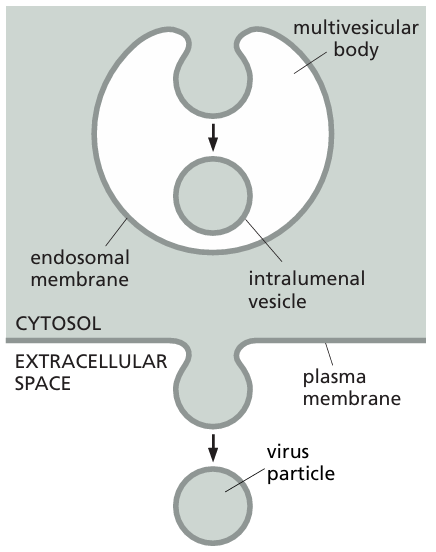
\includegraphics[width = 0.25\textwidth]{42}
	}
	\caption{Schematic Mechanism in macropinocytosis and multivesicular body formation}
\end{figure}

\paragraph{Transmembrane receptor proteins get endocytosed}

As \textbf{endosomes mature}, portions of their membrane invaginate into the lumen and pinch off, forming \textbf{internal vesicle}s. These maturing endosomes are called \textbf{\gls{multivesicular-body}} due to their distinctive appearance. A key role of MVBs is to to \textbf{hide away ubiquitylated membrane proteins} (like activated EGF receptors) into these intralumenal vesicles. This process ensures that the proteins are isolated from the cytosol, stopping any further signaling and making them fully accessible to lysosomal hydrolases. \textbf{See fig. \ref{sequestration}} \\
\indent Before the vesicles close, \textbf{the ubiquitin tag is removed and recycled}. Ultimately, when the multivesicular body fuses with a lysosome, \textbf{the enclosed vesicles and their contents are digested}. Without this internal sequestration (hiding away), parts of the membrane proteins exposed to the cytosol would escape degradation, since the lysosomal membrane itself is not broken down.

\begin{RemarkWithTitel}{ESCORT protein complexes}
	\gls{ESCRT}
	The ESCRT (Endosomal Sorting Complex Required for Transport) protein complexes (ESCRT-0, -I, -II, -III) play a crucial role in \textbf{sorting ubiquitylated membrane proteins into the intralumenal vesicles of multivesicular bodies}. Without proper ESCRT function, these receptors may continue to signal inappropriately, potentially contributing to diseases like \textbf{cancer}. Note that \textbf{ESCRT proteins are recruited from the cytosol to specific domains on the endosome membrane}, where they bind to PI(3)P lipids and ubiquitylated cargo proteins.
\end{RemarkWithTitel}

\begin{figure}[H]
	\centering
	\subfigure[Sorting of endocytosed membrane proteins into the intralumenal vesicles of a multivesicular body.]{
		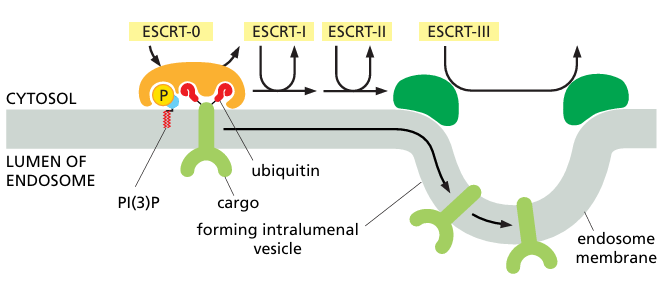
\includegraphics[width = 0.48\textwidth]{41}
	}
	% Second subfigure
	\subfigure[The sequestration of endocytosed proteins into intralumenal vesicles of multivesicular bodies.]{
		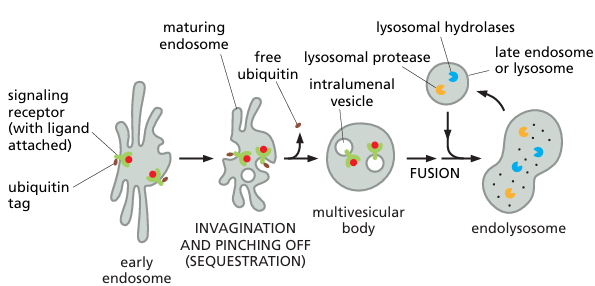
\includegraphics[width = 0.48\textwidth]{40}
		\label{sequestration}
	}
	\caption{ESCRT Protein Complexes Mediate the Formation of Intralumenal Vesicles in Multivesicular Bodies}
\end{figure}
Receptors behave differently depending on their type. Most are recycled back to their original membrane area, some are sent to a different area through \textbf{\gls{transcytosis}}, and others are degraded in lysosomes. Note that \textbf{the transcytotic pathway is not direct}. Therefore the receptors move first to en early endosome and then to a recycling endosome. Many \textbf{receptors possess sorting signals} that guide them into the appropriate transport pathway. \\
\\
\textbf{Cells can regulate the release of membrane proteins from recycling endosomes}, thus adjusting the flux of proteins through the transcytotic pathway according to need. For example in response to \textbf{insulin}, they can release stored glucose transporters. 
\begin{figure}[H]
	\centering
	\subfigure[Possible fates for transmembrane receptor proteins that have been endocytosed.]{
		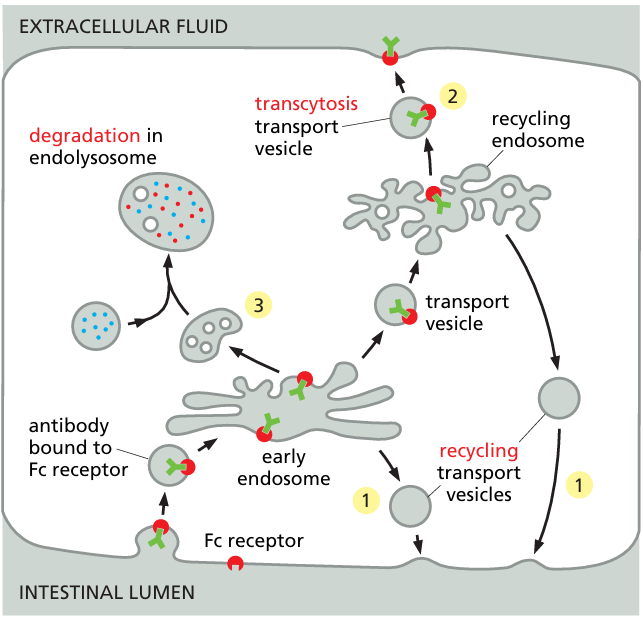
\includegraphics[width = 0.45\textwidth]{43}
	}
	% Second subfigure
	\subfigure[Storage of plasma membrane proteins in recycling endosomes.]{
		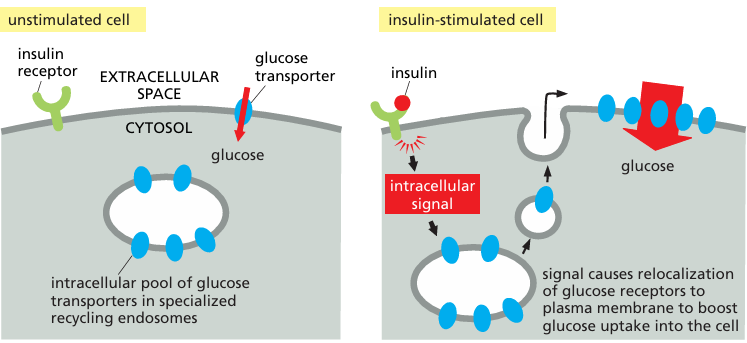
\includegraphics[width = 0.5\textwidth]{44}
		\label{sequestration}
	}
	\caption{Recycling Endosomes Regulate Plasma Membrane Composition}
\end{figure}



\subsection{Exocytosis}
Vesicles from the trans-Golgi network (TGN) deliver membrane and soluble proteins to the cell surface through exocytosis, replenishing the plasma membrane and releasing secreted proteins.\\
\indent All cells use a \textbf{\gls{constitutive-secretory-pathway}} for continuous protein export. \textbf{Specialized cells} also have a \textbf{\gls{regulated-secretory-pathway}}, where proteins are stored in vesicles and released on demand, such as hormones or neurotransmitters. 
\begin{figure}[H]
	\centering
	\subfigure[The three best-understood pathways of protein sorting in the trans Golgi network.]{
		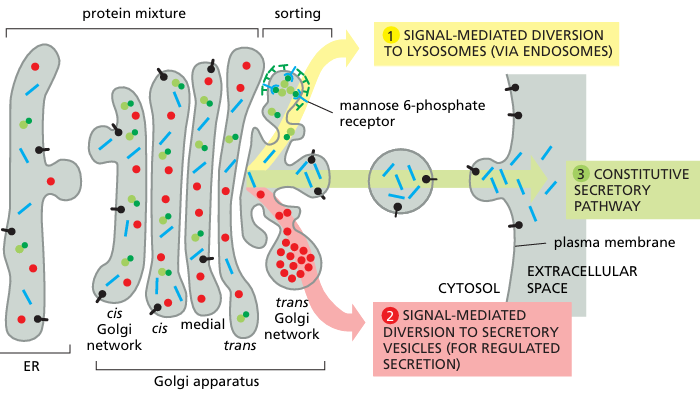
\includegraphics[width = 0.7\textwidth]{45}
	}
	% Second subfigure
	\subfigure[Exocytosis]{
		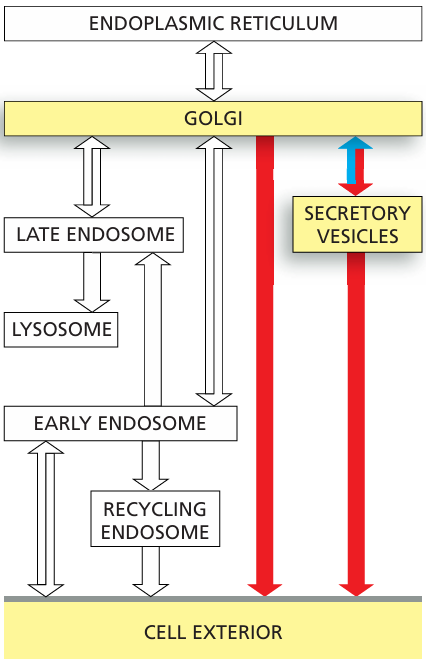
\includegraphics[width = 0.25\textwidth]{46}
	}
	\caption{Transport from the Trans Golgi Network to the Cell Exterior: Exocytosis}
\end{figure}
Note that all cell capable of regulated secretion must \textbf{separate at least three classes of proteins} before they leave the TGN, those destined for lysosomes (via endosomes, proteins tagged with M6P), those destined for secretory vesicles, and those destined for immediate delivery to the cell surface (\textbf{default pathway}: does not require a particular signal). \\
\indent In an \textbf{unpolarized cell}, such as white blood cells or a fibroblast, it seams that particularly any produced protein is carried by the constrictive pathway. While in \textbf{polarized cells} the options are more diverse :). \\
\\
Cells that are specialized to secreting some of their products rapidly on demand concentrate and store these products in \textbf{secretory vesicles}. These vesicles are often called \textbf{densecore secretory granules} since they have a dense core visible in EM. \\
\indent These core is dense since the \textbf{secretory proteins often aggregate}. It is though \textbf{unclear} how the aggregates are packed into secretory vesicles. They uptake may \textbf{resemble phagocytosis} quite a bit. \\
\\
Initially, the \textbf{immature secretory vesicles} leaving the trans-Golgi network (TGN) contain loosely packed proteins and \textbf{resemble swollen Golgi cisternae}. \textbf{As they mature, these vesicles fuse, their contents become more concentrated}, and their \textbf{interiors acidify due to V-type ATPases}, which pump protons into the lumen.
\\
\indent\textbf{Membrane recycling helps return Golgi components} and further concentrates the contents of secretory vesicles. Clathrin-coated buds on immature vesicles mediate this retrieval process. \textbf{As a result, mature vesicles are densely packed} and ready to rapidly release their contents upon stimulation.\\
\indent This increase in concentration happens because:
\begin{itemize}
	\item \textbf{Membrane is continually recycled} from the immature vesicle back to the Golgi, reducing vesicle volume.
	\item \textbf{The vesicle lumen becomes more acidic} due to V-type ATPases, promoting condensation of the protein cargo.
\end{itemize}
Although the \textbf{total amount of protein remains constant} after vesicle formation, the \textbf{volume decreases}, leading to a \textbf{higher protein concentration}—a key step in preparing for rapid, efficient secretion.

\begin{figure}[H]
	\centering
	\subfigure[The formation of secretory vesicles.]{
		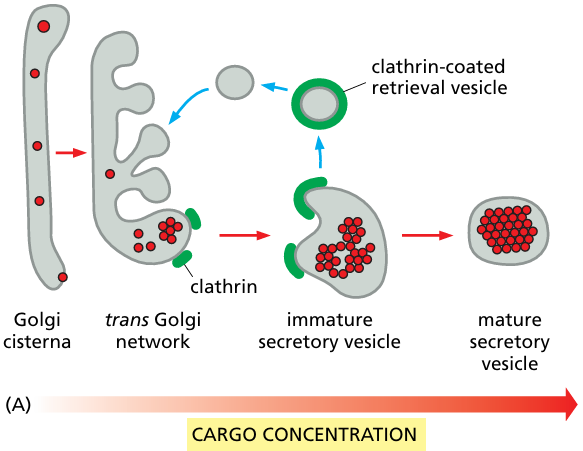
\includegraphics[width = 0.45\textwidth]{47}
	}
	% Second subfigure
	\subfigure[Exocytosis of secretory vesicles.]{
		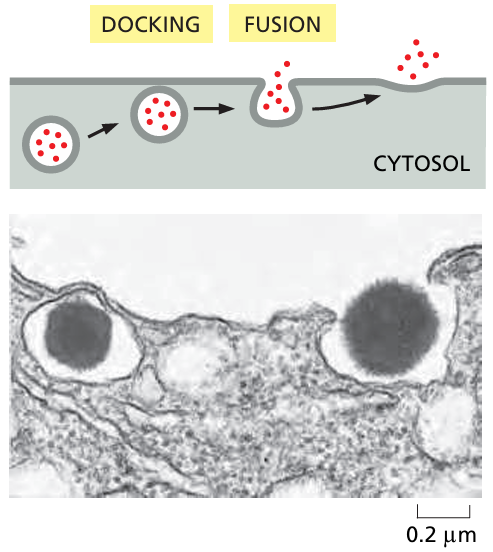
\includegraphics[width = 0.3\textwidth]{48}
	}
	\caption{Secretory Vesicles Bud from the Trans Golgi Network}
\end{figure}

\begin{RemarkWithTitel}{Proteolytic Processing of Secretory Proteins}
	As secretory vesicles mature, many secretory proteins are processed by proteolysis. Hormones, neuropeptides, and hydrolytic enzymes are often synthesized as inactive precursors that \textbf{must be cleaved to become active}.\\
	\indent Proteolytic cleavage occurs in the secretory vesicle or after secretion and helps:
	\begin{itemize}
		\item Activate short signaling peptides that couldn't otherwise be transported or packaged.
		\item Prevent premature activity of potentially harmful enzymes within the cell.
	\end{itemize}
	These precursor proteins are commonly synthesized as \textit{pre-pro-proteins}, or polyproteins, which are processed into one or multiple active peptides, depending on the cell type.
\end{RemarkWithTitel}

\paragraph{Exocytosis of synaptic vesicles}
Nerve and some endocrine cells have two types of secretory vesicles. One type, \textbf{dense-cored vesicles}, releases proteins and neuropeptides through the regulated secretory pathway. The other type, \textbf{synaptic vesicles} (about 50 nm wide), stores small neurotransmitters like acetylcholine, glutamate, glycine, and GABA for fast communication at synapses. When an action potential reaches the nerve terminal, \textbf{calcium enters the cell and triggers these vesicles to release their contents}.\\
\indent This \textbf{fast release is made possible by a priming step where SNARE proteins partially pair}. Complexins hold the SNAREs in this ready (metastable) state. When Ca2+ levels rise, synaptotagmin binds to the SNAREs and membrane lipids, displacing complexins and allowing full SNARE zippering. This opens a fusion pore, releasing neurotransmitters. Only a few vesicles are primed at a time, allowing rapid and repeated firing as new vesicles continuously dock and prepare for release.
\begin{figure}[H]
	\centering
	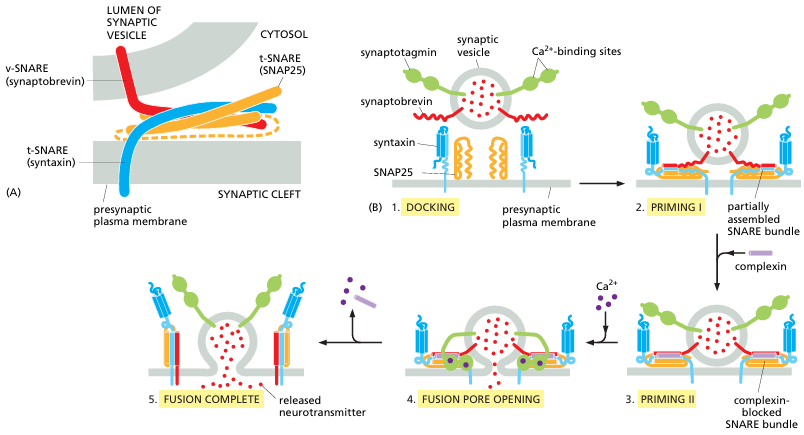
\includegraphics[width= \textwidth]{51}
	\caption{Exocytosis of synaptic vesicles.}
\end{figure}
To support rapid and repeated firing, \textbf{synaptic vesicles are quickly replenished through local recycling at the nerve terminal}, rather than being made in the cell body. New membrane components are first delivered to the plasma membrane, then retrieved by endocytosis. Instead of fusing with endosomes, most endocytic vesicles are quickly refilled with neurotransmitter and reused as synaptic vesicles.
\begin{figure}[H]
	\centering
	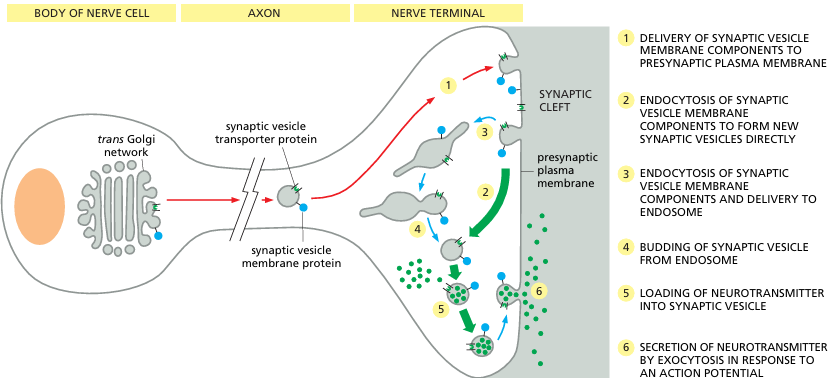
\includegraphics[width= 0.9   \textwidth]{50}
	\caption{The formation of synaptic vesicles in a nerve cell.}
\end{figure}

\paragraph{Sorting plasma membrane proteins in polarized epithelial cell}
In polarized epithelial cells, which have distinct \textbf{apical} and \textbf{basolateral} membrane domains, plasma membrane proteins are sorted by two main mechanisms:

\begin{enumerate}
	\item \textbf{Direct Sorting at the Trans-Golgi Network (TGN):} \\
	Proteins are sorted in the TGN and transported directly to either the apical or basolateral membrane. Sorting signals and mechanisms such as lipid rafts (e.g., for GPI-anchored proteins) help target proteins to the correct domain.
	
	\item \textbf{Indirect Sorting via Transcytosis:} \\
	Some proteins are first delivered to one membrane domain (typically the basolateral side), then internalized and redirected to the correct domain (e.g., apical) through endosomal transport.
\end{enumerate}

\begin{figure}[H]
	\centering
	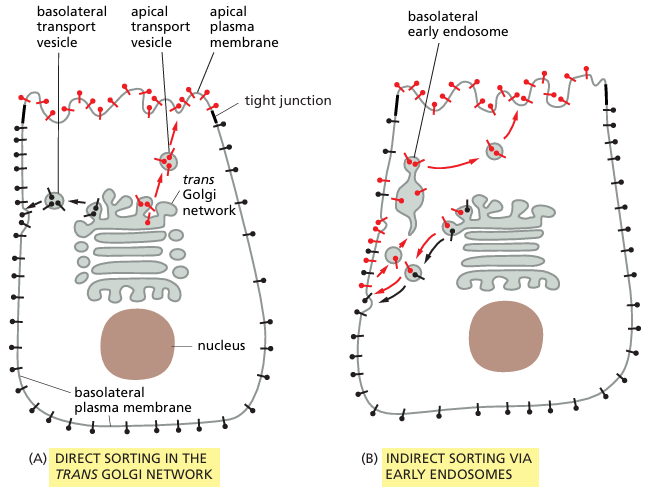
\includegraphics[width= 0.55\textwidth]{49}
	\caption{Two ways of sorting plasma membrane proteins in a polarized epithelial cell.}
\end{figure}

\printglossaries	
\end{document}	